\documentclass{article}

\usepackage{epcc}
\usepackage{url}
\PassOptionsToPackage{hyphens}{url}
\usepackage[colorlinks=false, hidelinks]{hyperref}
\usepackage{amsmath}
\usepackage[toc,page]{appendix}
\usepackage[table]{xcolor}
\usepackage[marginparsep=30pt]{geometry}
\usepackage{stmaryrd}
\usepackage{algorithm}
\usepackage{algorithmic}
\usepackage{tikz}
\usepackage{pgfplots}
\usepackage{tabu}
\usepackage{longtable}
\usepackage{tabularx}
\usepackage{listings}
\usepackage{fancyref}
\usepackage{relsize}
\usepackage{float}
\usepackage{graphicx}
\usepackage{subcaption}
\usepackage{diagbox}
\usepackage{multirow}
\usepackage{slashbox}
\usepackage{graphics}
\usepackage{booktabs}
\usepackage{natbib}
\usepackage{csquotes}

\usetikzlibrary{%
    arrows,
    arrows.meta,
    decorations,
    backgrounds,
    positioning,
    fit,
    petri,
    shadows,
    datavisualization.formats.functions,
    calc,
    shapes,
    shapes.multipart,
    matrix,
    plotmarks
}

\usepgfplotslibrary{fillbetween, statistics, dateplot}

\pgfplotsset{%
  compat=1.3,
  every non boxed x axis/.style={%
  enlarge x limits=false,
  x axis line style={}%-stealth},
  },
  every boxed x axis/.style={},
  every non boxed y axis/.style={%
  enlarge y limits=false,
  y axis line style={}%-stealth},
  },
  every boxed y axis/.style={},
}

\renewcommand{\labelenumii}{\theenumii}
\renewcommand{\theenumii}{\theenumi.\arabic{enumii}.}

\bibliographystyle{plainnat}
\bibpunct{(}{)}{;}{a}{,}{,}

\begin{document}

\pagenumbering{roman}

\title{Deep Learning on SpiNNaker: Report}
\author{Jonas Fassbender \\ \textit{jonas@fassbender.dev}}
\date{}

\makeEPCCtitle

\newpage

\begin{abstract}
\end{abstract}

\newpage

\tableofcontents

\newpage

\pagenumbering{arabic}

\section{Introduction} % {{{
\label{sec:intro}

According to the SpiNNaker project's website:
\begin{displayquote}
  SpiNNaker is a novel massively-parallel computer
  architecture, inspired by the fundamental structure and
  function of the human brain, which itself is composed of
  billions of simple computing elements, communicating
  using unreliable spikes \citep{spinn_proj}.
\end{displayquote}

SpiNNaker is a digital neuromorphic computer architecture,
designed to model the human brain.
This is rather a gross simplification of what SpiNNaker was
designed for.
Understanding the human brain is one of the biggest
frontiers of science and there are many ideas on how one
can model a complex and still mostly unknown structure such
as the human brain.
Therefore, there are many different proposed neuromorphic
computer architectures and ideas on how to model the human
brain, from early analogue approaches for vision systems
like presented in \citet{mead1989} to large scale digital
architectures like Blue Brain \citep{markram2006}; all
aiming to implement different types of neurons and models
of the human brain efficiently \citep{furber_et_al_2007}.

SpiNNaker is an architecture for the large scale and
real-time modeling of spiking neural networks
\citep{furber_et_al_2006, furber_et_al_2006b,
  furber_et_al_2007}.
\citet{maass1997} describes spiking neural networks as the
third generation of neural networks.
Unlike the second generation neural networks---which we
will deal with in the dissertation project here reported on
in the form of deep learning neural networks---spiking
neural networks incorporate a concept of time in their
action potentials (spikes).
Neural networks of the second generation do not have a
concept of time and fire every time they are activated.
Spiking neural networks are derived from evindence
collected from biological neural systems; they are therfore
more closely representing neural systems of biological
life than deep learning neural networks \citep{maass1997}.

The SpiNNaker chip is a ARM multiprocessor chip having 18
cores, with a Network-on-Chip system for
communication between cores \citep{furber_et_al_2007,
  spinn_proj}.
Each core can model up to 1000 spiking neurons.
The spiking neurons in the neural network communicate with
spike events \citep{furber_et_al_2007}.
Spike events are---like their biological
counterpart---inheritently unstable and small.
This is represented in the interconnection hardware.
Small packets (40 or 72 bits) can be send, without
guarantee of successful arrival.
Even without this guarantee, on can still perform
meaningful computations on SpiNNaker and fault detection
and recovery mechanisms are implemented \citep{spinn_proj}.
One can connect many SpiNNaker chips together, to build a
masively parallel and energy efficient supercomputer that
is able to run up to a billion spiking neurons in real time
\citep{furber_et_al_2007}.
Photos of the SpiNNaker hardware can be found in
Appendix~\ref{sec:spinn_photos}.

SpiNNaker is targeted at three main areas of research:
(\romannumeral 1) neuroscience: understanding the human
brain, (\romannumeral 2) robotics: low power hardware for
implementing neural decision systems and
(\romannumeral 3) computer science: new approach to
supercomputing and massive parallelism \citep{spinn_proj}.
The dissertation project, which this paper reports on,
will concern itself with (\romannumeral 3) and one of the
research areas of computer science, which has emerged as
a driving force behind advancements in many fields and for
many tasks like speech and image recognition, drug
discovery and genomics: deep learning
\citep{lecun_et_al_2015}.

While deep learning is a promising field and deep neural
networks at the center of important advancements, like
described above, they face a major problem: the sheer
amount of computation needed for training them.
Researchers at OpenAI have estimated, that the amount of
computation needed for training state of the art deep
neural networks increases exponentially, doubling every
3.4 months \citep{openai2019}.
In order to cope with such unprecedented amounts of
computation and energy needed, the search for specialized
hardware is well underway.
Current state of the art hardware for accelerating the
training of deep neural networks are ASICs like TPUs and
general purpose GPUs \citep{tpus, mittal_et_al_2019}.

The goal of the dissertation project that is introduced in
this paper, will be to analyze if SpiNNaker could be an
energy efficient, scalable and fast alternative to the
above mentioned hardware.
Since deep neural networks are derived from the human
brain and nerve system \citep{goodfellow2016} and SpiNNaker
was designed to model the human brain, it seems rather
probable, that SpiNNaker will be a good target for
accelerating the training of deep neural networks.

This paper concerns itself with the dissertation project:
``Deep Learning on SpiNNaker'', which will be conducted in
the period from May 2019 to August 2019 as the final work
of the author to achieve his Master of Science in
High Performance Computing with Data Science from the
University of Edinburgh.
The report is mostly a summary of the preliminary work
conducted in the months before the actual work on the
disseration will be conducted.

The finindings of the preliminary work and the changes made
to the original project scope are the focal point of this
report.
The original title of the disseration project was ``A
Tensorflow Backend to SpiNNaker'', but the preliminary work
conducted to this point show, that the scope will be
redirected from implementing a backend for tensorflow---a
library for running fast linear algebra operations on
distributed, heterogenous systems, mainly designed for
implementing computationally demanding machine learning
algorithms like deep learning in a fast manner
\citep{tf2015}---to an approach focused on implementing
deep learning directly on SpiNNaker.
Because of SpiNNaker's specialized design, which works
rather contrary to that of tensorflow and current hardware
trends for building accelerators for deep learning,
interfacing between SpiNNaker's runtime and tensorflow was
deemed too difficult and not beneficial.
Instead, this dissertation aims at implementing deep
learning directly on SpiNNaker, probably providing an
interface designed in the likes of the well known deep
learning library Keras \citep{keras}.
\citet{proj} shows the original disseration project's
scope.

This paper starts with presenting the final project
proposal, in particular focusing on the benchmark to be
conducted in Section~\ref{sec:proposal}.
Afterwards related work is presented in
Section~\ref{sec:related_work}.
The main focus lies on presenting papers with benchmarks
we can compare our implementation against.
The paper continues by giving a work plan in
Section~\ref{sec:work_plan}, before presenting a risk
analysis in Section~\ref{sec:risk_analysis}.
Afterwards the preliminary findings outlined above are
disscussed in more depth in Section~\ref{sec:prelim}.
At last Section~\ref{sec:review} will contain a review of a
related dissertation project done in 2018:
``Deep Learning Performance on Different Architectures'' by
Spyro Nita \citep{nita_2018}.

% }}}

\section{Final Project Proposal} % {{{
\label{sec:proposal}

This section will begin by giving an outline of the initial
project proposal.
The preliminary findings given in Section~\ref{sec:prelim}
lad us to abandon the initial project proposal.
The updated project proposal is given.
The benchmark with which we will compare our deep learning
implementation on SpiNNaker with other hardware platforms
and deep learning libraries is presented.

The final project proposal will differ from the initial one
in two meaningful ways: (\romannumeral 1) we will implement
deep learning algorithms and layers directly on SpiNNaker,
instead of implementing a tensorflow backend (see
Section~\ref{sec:prelim}) and (\romannumeral 2) a different
benchmark to measure the performance of SpiNNaker.
While at first, implementing a tensorflow backend in order
to enable deep learning on SpiNNaker seemed wise: low
level linear algebra operations based on which deep
learning algorithms run, instead of having to implement
them directly.
The discrepancy between tensorflow's architecture and
SpiNNaker's was deemed too big to overcome and to get a
working deep learning neural network running in the limited
amount of time for doing the dissertation was estimated to
be impossible.
Concerning (\romannumeral 2), the benchmark proposed by the
initial proposal was to benchmark our native deep learning
implementation against the snn toolbox
\citep{rueckauer_et_al_2017}.
The snn toolbox allows taking pre-trained deep neural
networks and convert them to spiking neural networks, which
then can be deployed on SpiNNaker.
The problem with this benchmark is the fact, that only
pre-trained deep neural networks can be used and only
inference would be possible on SpiNNaker.
We do not aim at doing the rather inexpensive inference
(at least compared to the training), rather we want to
use SpiNNaker where it would be needed more: training
a deep neural network---a computationally very costly
operation (see Section~\ref{sec:intro}).

Instead of benchmarking against the snn toolbox, we intend
to go for a much more ambitious benchmark.
We want to benchmark the performance of our implementation
on SpiNNaker against other state of the art hardware and
software libraries for deep learning based on a model for
computer vision---a very popular problem domain for deep
learning, providing many good benchmarks we can compare
against (see Section~\ref{sec:related_work}).

Currently, the most famous and probably biggest challenge
for benchmarking computer vision models is the
ImageNet Large Scale Visual Recognition Challenge (ILSVRC),
based on the ImageNet dataset.
The ImageNet dataset consists of more than 14 million
images, organized according to the WordNet hierarchy into
over 21 thousand so called synsets (synonym sets)
\citep{imagenet, wordnet}.
The ILSVRC is an annual competition running since 2010.
It has produced many famous models, e.g. AlexNet, VGG16 or
ResNet-50 \citep{alexnet, simonyan_et_al_2014,
  he_et_al_2015}.
We intend to benchmark by training the most complex of
these three models: ResNet-50.
The benchmark will be to train ResNet-50 with 1000
categories (1.28 million images) of the ImageNet dataset
(setting of the ILSVRC 2012) and measure the time it takes
to finish the training.
The top-1 accuracy of the model is evaluated on 50,000 test
images and should be at least 74.9\%, in order to compare
it to the other benchmarks presented in
Section~\ref{sec:related_work}.

In conclusion, our final project proposal will be
implementing deep learning algorithms directly on
SpiNNaker, instead of providing a backend to tensorflow.
We will benchmark this implementation and SpiNNaker against
other benchmarks based on state of the art deep learning
libraries and accelerators for fast training of neural
networks, instead of benchmarking our implementation
against the snn toolbox.
For this benchmark we will train the famous ResNet-50 model
based on the settings described above and compare our
results against the results others generated with the same
setting but with different libraries and hardware, which
are presented below.

% }}}

\section{Related Work} % {{{
\label{sec:related_work}

This section will foucus itself with related work important
for the final project proposal of ``Deep Learning on
SpiNNaker''.
The main focus lies on benchmarks, with wich we can compare
our impelementation on SpiNNaker with state of the art
libraries and---more importantly---hardware.
Further literature of importance for this project, e.g.
\citet{he_et_al_2015}, \citet{goodfellow2016} or
\citet{imagenet}, can be found in the References.

The benchmark settings described in the previous chapter
are the image classification benchmark for training deep
learning models of the recently launched MLPerf benchmark
project.
The MLPerf benchmark was proposed, to ensure fair
performance comparisons between various hardware and
software libraries for deep learning
\citep{mattson_et_al_2019}.
We intend to stick to the rules of the MLPerf benchmark.
If the dissertation project will succeed as planned, we
will submit our timing results to the MLPerf Training
benchmark v0.7, which is due on the 21st of February 2020.
The results of MLPerf Training v0.6 can be found at
\url{https://mlperf.org/training-results-0-6/}.
Currently the fastest system for the image classification
benchmark is based on tensorflow and 1024 TPUv3s.
It is able to finish in 1.28 minutes.
Besides the MLPerf benchmark, which is quite new, there
are a few older papers which use a similar setting for
benchmarking their systems.
These papers and their results are listed in
Table~\ref{tab:benchmarks}.

\begin{table}
\begin{center}
\begin{tabu}{|l|l|l|l|l|}
\hline
paper &processor/accelerator &\# &library &time \\
\hline
\citet{he_et_al_2015} &Tesla P100 &8 &caffe &29 hours \\
\citet{goyal_et_al_2017} &Tesla P100 &256 &caffe2 &1 hour \\
\citet{smith_et_al_2017} &TPU pod &1 &tensorflow &30 minutes \\
\citet{akiba_et_al_2017} &Tesla P100 &1024 &chainer &15 minutes \\
\citet{you2017} &Xeon Phi KNL &2048 &caffe &14 minutes \\
\citet{jia_et_al_2018} &Tesla P40 &2048 &tensorflow &6.6 minutes \\
\citet{mikami_et_al_2018} &Tesla V100 &2176 &NNL &3.7 minutes \\
\hline
\end{tabu}
\end{center}
\caption{Selected timings from benchmarks other than MLPerf
  with a similar setting. None can beat the fastest system
  from the MLPerf benchmark, which is not surprising,
  given the fast pace of improvements in both hardware
  and software for deep learning and the fact, that the
  MLPerf benchmark results are the most recent.}
\label{tab:benchmarks}
\end{table}

% }}}

\section{Work Plan} % {{{
\label{sec:work_plan}

% }}}

\section{Risk Analysis} % {{{
\label{sec:risk_analysis}

% }}}

\section{Preliminary Findings} % {{{
\label{sec:prelim}

% main problem will be programming

% => minimize everything that is not programming
%    (benchmarking: use other benchmarks, ...)

% tf backend too difficult (XLA, linear algebra not what
% spinnaker was designed for)

% implement subset of keras api (or at least a keras like
% python api) to make benchmark possible

% }}}

\section{Deep Learning Performance on Different % ... {{{
  Architectures: Review}
\label{sec:review}

This section will concern itself with a review of the
dissertation of Spyro Nita, which he did for earning his
Master of Science in High Performance Computing with Data
Science at the University of Edinburgh:
``Deep Learning Performance on Different Architectures''
 \citep{nita_2018}.
First, a summary of his dissertation will be given, before
the review of his work is presented.
The review will start by looking at how well the context
of the dissertation is explained and how well the scope
of the dissertation's problem is defined.
The last part of the review will be the consideration of
the dissertation's layout and formatting.
After the review, the importance of the dissertation for
``Deep Learning on SpiNNaker'' will be discussed and
evaluated.

\citet{nita_2018} concerns itself with measuring the
computational performance of two different approaches for
training deep neural networks: (\romannumeral 1)
distributed training using GPUs and (\romannumeral 2)
distributed training using CPUs.
The dissertation is a work derived of the efforts of
Team EPCC at the Student Cluster Competition at the
International Supercomputing Conference 2018, held in
Frankfurt, where Team EPCC competed against other teams by
building a small supercomputing cluster and running various
benchmarks on it, to see which team built the best
supercomputing cluster.
One of these benchmarks concerned itself with measuring the
performance of training a deep neural network on the
clusters, which is picked up in \citet{nita_2018} and
represents the benchmark for approach (\romannumeral 1).


The benchmark is based on the famous ImageNet dataset, like
the ILSVRC (see Section~\ref{sec:proposal}).
Contrary to the ILSVRC, the benchmark for the Student
Cluster Competition only concerns itself with the
throughput of images during training and not with the
accuracy of the trained models.
The throughput is measured in images per second.
Only if two teams should have the same throughput during
training is the training accuracy taken into account as
the secondary criterion for tie-breaking.
The teams participating in the Student Cluster Competition
had to train the VGG16 deep neural network---a famous
model architecture introduced in the ILSVRC 2014 by
researchers from Oxford University
\citep{simonyan_et_al_2014}---on 1000 synsets containing
1.2 million images.
The main limitation for the clusters were their power
budget of 3kW and---for the ImageNet benchmark---a maximum
runtime of three hours \citep{nita_2018}.

\citet{nita_2018} compares the throughput of the
supercomputing cluster of Team EPCC for the performance of
a distributed GPU system against Cirrus---a supercomputer
hosted by the EPCC---for the performance of a distributed
CPU system \citep{cirrus}.

Concerning the results of \citet{nita_2018}, two major
problems were encountered: (\romannumeral 1) cluster
damage and failure of the Team EPCC cluster shortly before
the competition and (\romannumeral 2) the fact that the CPU
benchmark on Cirrus could not be distributed over multiple
backend nodes.
Fortunately benchmarks were done on the Team EPCC cluster,
before its failure and \citet{nita_2018} presents the
results of using the first node of the cluster with six
NVIDIA V100 GPUs.
Concerning (\romannumeral 2), \citet{nita_2018} presents
the results for a single backend node and assumes that
Cirrus would be able to linearly scale to multiple backend
nodes, when comparing the two clusters.
The single node of the Team EPCC cluster with its six
NVIDIA V100 GPUs generates a throughput of 2,052 images per
second, while a single backend node of Cirrus (two Intel
Xeon E5-2695 processors, each with 18 physical cores) can
generate a throughput of just 18 images per second.
Assuming linear scaling over multiple backend nodes of
Cirrus, 21 nodes would be needed for the throughput of a
single NVIDIA V100 GPU.
\citet{nita_2018} concludes that GPUs offer a significant
advantage compared to CPUs, when it comes to training
deep neural networks.

The dissertation starts with an introduction, which
includes a description of the dissertation's layout.
The second chapter concerns itself with a description of
convolutional neural networks for image classification,
describing ImageNet and VGG16 as a special convolutional
neural network.
Chapter three describes everything concerning the Student
Cluster Competition, including the benchmarks, rules and
various features of the Team EPCC cluster, including the
used hardware, operating system and other important
software libraries.
It also describes the difficulties and hardware damage to
the cluster and---concerning the ImageNet benchmark---how
the images were preprocessed and reformatted to the
TFRecord format \citep{tf2015}.
Chapter four concerns itself with the optimization of the
VGG16 neural network, mainly through different parameters
which are passed to tensorflow, which is used for
implementing VGG16.
It thoroughly describes how one can distribute training
across multiple GPUs.
The benchmark for the Student Cluster Competition is
described and analyzed, as is the benchmark for Cirrus.
The chapter ends by comparing both.
\citet{nita_2018} concludes by summarizing the results
presented in chapter four and gives an outline for future
work, which could shed more light on the performance of
GPU and CPU clusters for training deep neural networks.
The two main points of emphasis for future work presented
are: (\romannumeral 1) scaling training to hundreds of
CPU nodes \citep[see e.g.][for distributing training onto
multiple CPUs]{you2017} and (\romannumeral 2)
comparing power consumption of CPU nodes against GPU nodes.

The best thing to say about \citet{nita_2018} is how well
the whole experience of the Student Cluster Competition is
communicated by the author.
\citet{nita_2018} does not simply give a description of
everything that is important for the benchmark, but gives
a very conclusive and elaborate review of the whole
competition.
It serves as a red line throughout the whole dissertation.

Chapter four contains the benchmark and its results.
It is a conclusive chapter and well annotated with useful
references.
The difficulties of the environment are clearly described
and while there were failures and the benchmarks on both
the cluster of Team EPCC and Cirrus are not optimal, these
difficulties are discussed openly and the presented results
are sensible.

Overall, \citet{nita_2018} describes the context and
problem scope well.
Its only problem is, it does not make it easy for the
reader to see that.
The layout can only be described as cluttered and a few
passages and paragraphs are simply unnecessary.
For example, Chapter~3.4 does not belong in the chapter
that concerns itself with the Student Cluster Competition,
if it belongs into the dissertation at all.
While the chosen data format could be seen as an
optimization and therefore should be described in chapter
four, problems during the download before the competition
are irrelevant to the benchmark.
Also chapter three and two could be swapped, which would
have made for an easier introduction to the dissertation,
where one is first confronted by the whole context and
rather gentle chapter about the Student Cluster
Competition, instead of by a description of convolutional
neural networks and ImageNet.
The first paragraph of the introduction to the dissertation
is just weird and seems to pay homage to
\citet{goodfellow2016}, which also starts with a similarly
weird introduction about Greek mythology and the craving of
humankind for thinking machines; absolutely irrelevant for
both: benchmarking deep neural networks and deep learning
in general.

A second point of critique could be the absence of a
chapter on related work, which gives a rough overview of
other, comparable benchmarks.
Some other benchmarks, like \citet{you2017}, are referenced
in the dissertation, but the reader does not get a general
overview over what else is out there.

\citet{nita_2018} and ``Deep Learning on SpiNNaker''
overlap in their problem scope, in the sense that both
concern itself with benchmarking the training speed of
deep neural networks.
Both focusing on image recognition based on the ImageNet
dataset.
While probably not directly important for the benchmark
conducted as part of ``Deep Learning on SpiNNaker'',
since \citet{nita_2018} benchmarks the VGG16 model and
``Deep Learning on SpiNNaker'' will focus on ResNet-50
(see Section~\ref{sec:proposal}),
\citet{nita_2018} still provided a great first point of
reference for the literature review done so far.

% }}}

\bibliography{library.bib}
\addcontentsline{toc}{section}{References}


\begin{appendices}
\section{Photos of SpiNNaker}
\label{sec:spinn_photos}

\begin{figure}[H]
  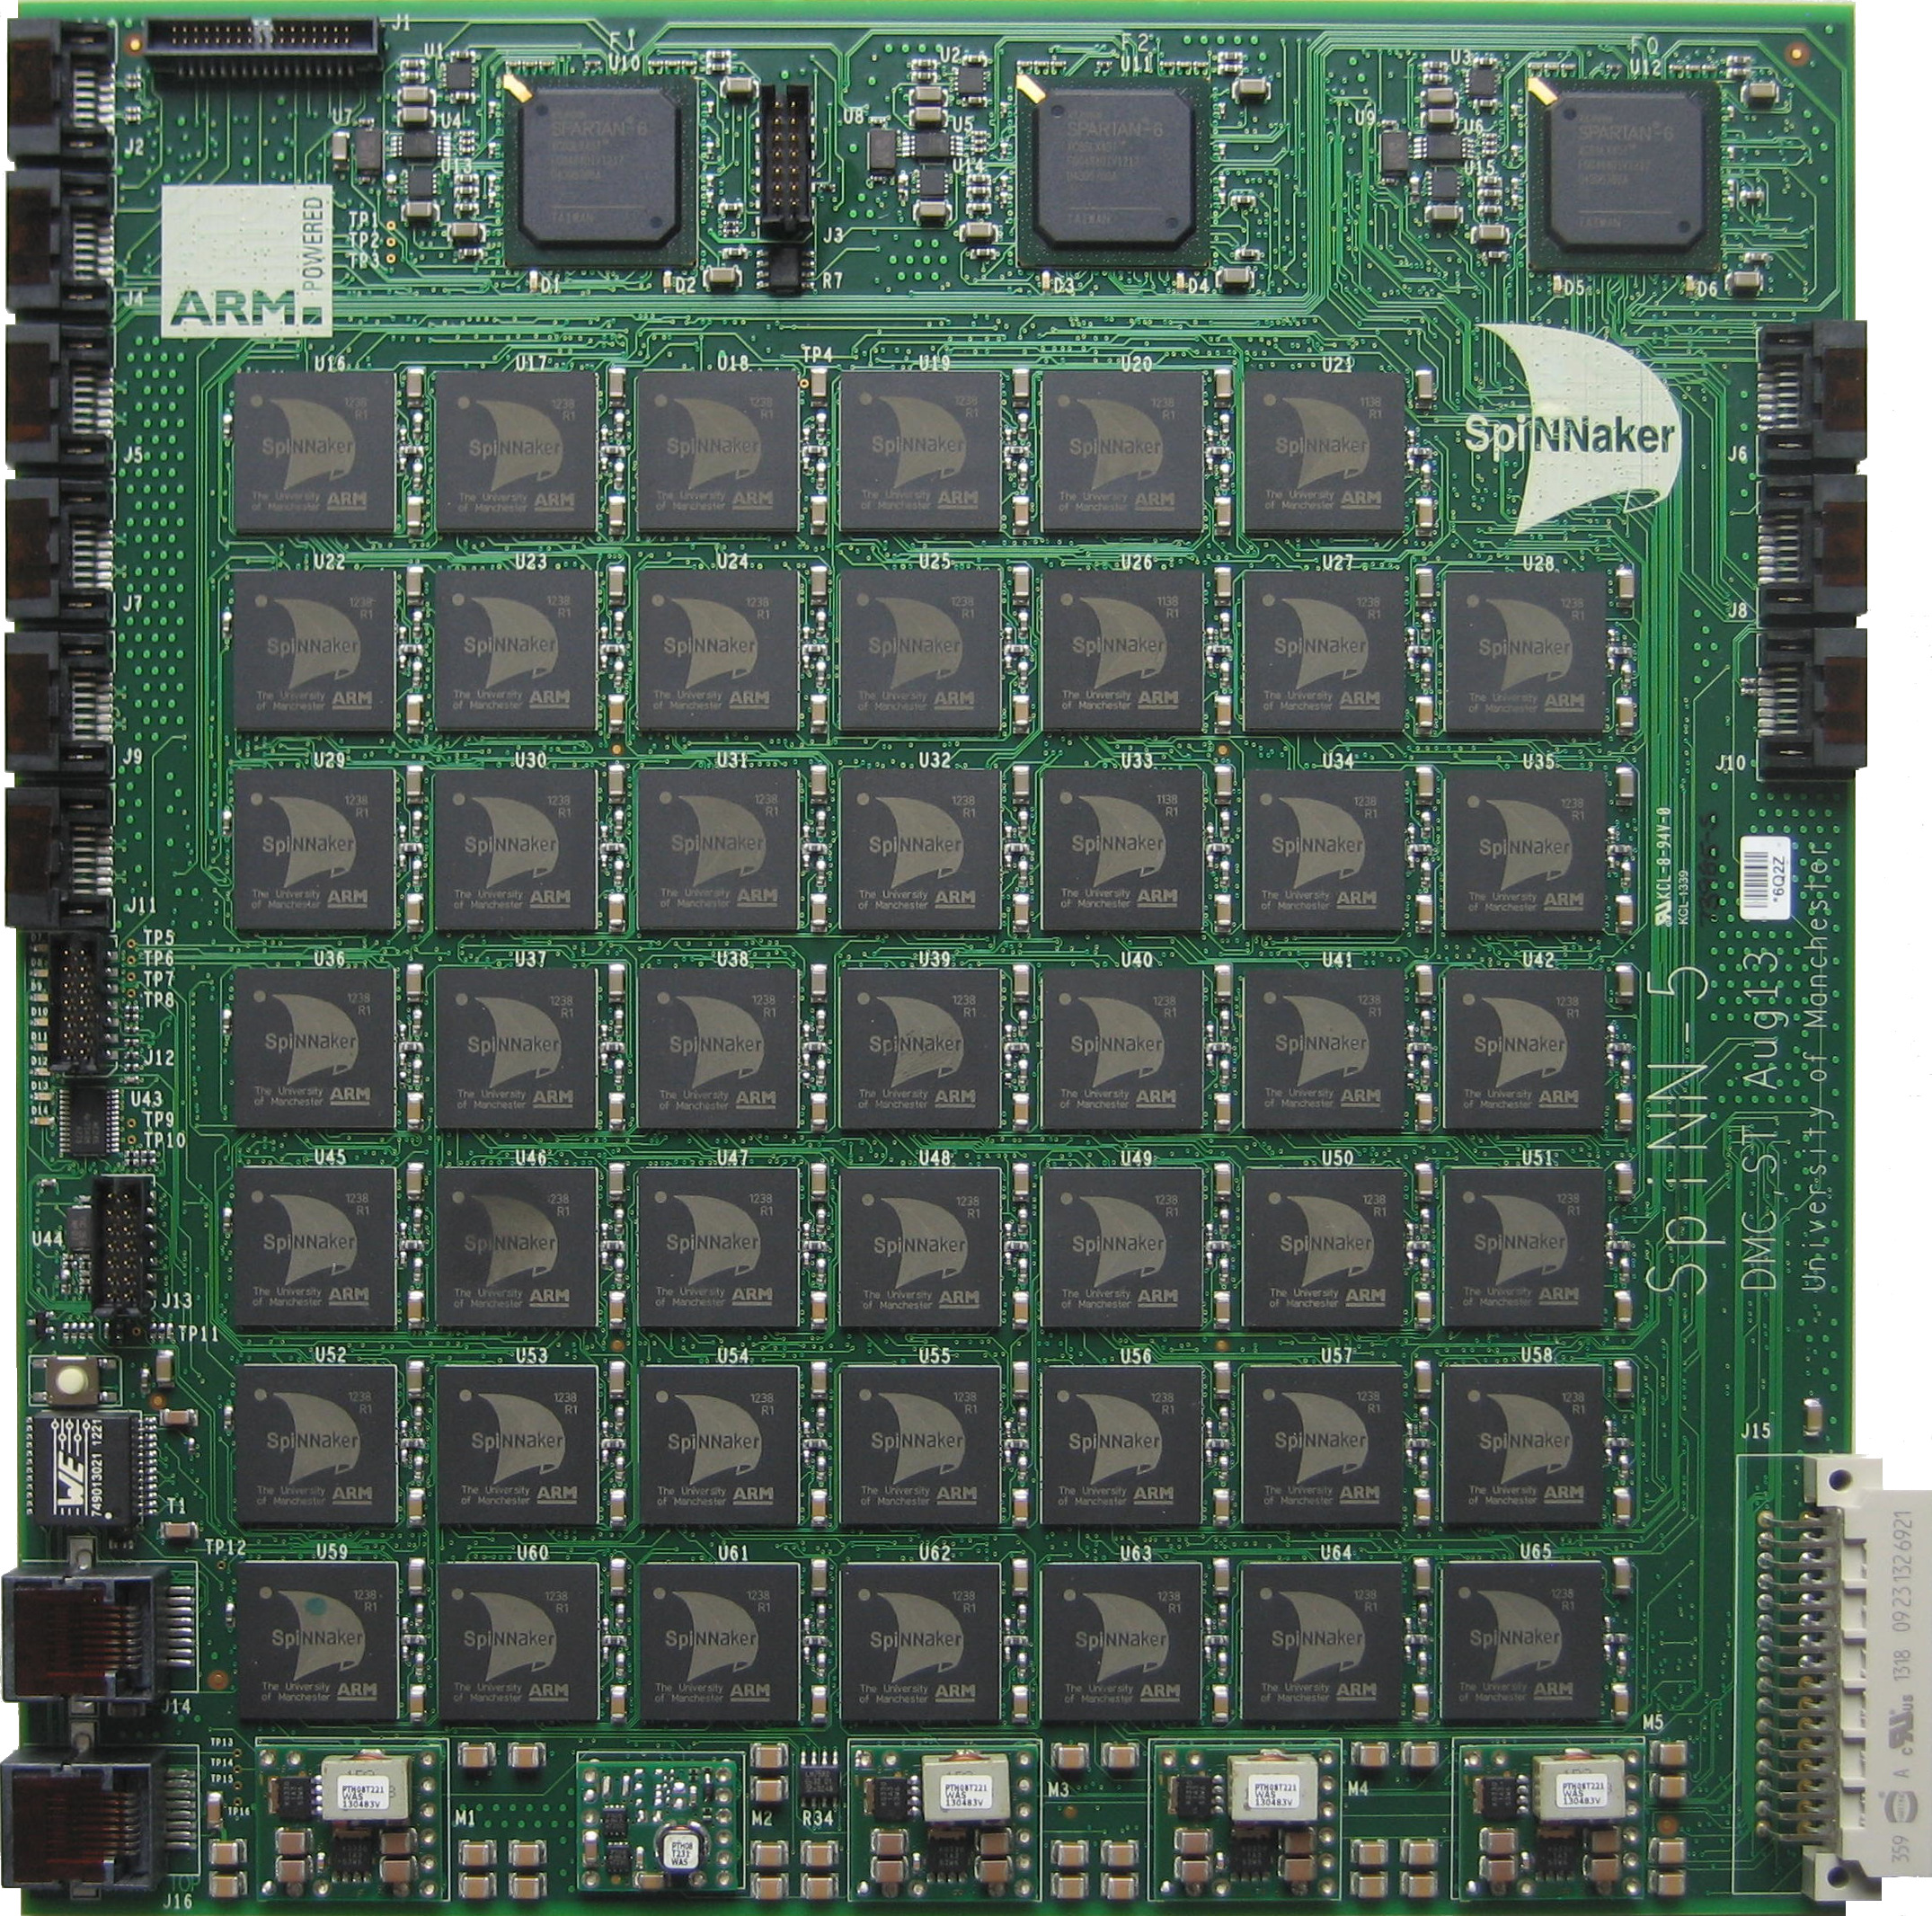
\includegraphics[width=\linewidth]{spinnakerBoard.jpg}
  \caption{A single SpiNNaker board with 48 SpiNNaker
    chips. Each chip has 18 cores.}
\end{figure}

\begin{figure}[H]
  \includegraphics[width=\linewidth]
    {SpiNNaker_9cabinets.jpg}
  \caption{The one million core machine in Manchester.
    It is capable of running up to one billion spiking
    neurons in real-time.}
\end{figure}

\end{appendices}

\end{document}
